\documentclass{article}
\usepackage[margin=3cm]{geometry}
\usepackage[utf8]{inputenc}
\usepackage{float}
\usepackage{graphicx} % Required for figures
\usepackage{anysize}
\usepackage{booktabs}
\usepackage{hyperref}
\usepackage{fontawesome5}
\usepackage{multirow}
\usepackage{array}
\usepackage[export]{adjustbox}
\usepackage{marvosym}

\title{\bfseries\Huge CV}
\begin{document}
\section*{\Huge CV}
\subsection*{Thomas Krogh Lohse}

%\par\noindent\rule{\textwidth}{1pt}
\begin{tabular}{m{0.4735\textwidth}m{.4735\textwidth}}
    \toprule%\\[-10pt]
    \href{https://goo.gl/maps/SZ6nwvdFf59X1VvR7}{\faIcon{map-marker-alt}\large~Thulevej 8 3th, Aalborg SØ 9210} & \multirow{6}{*}{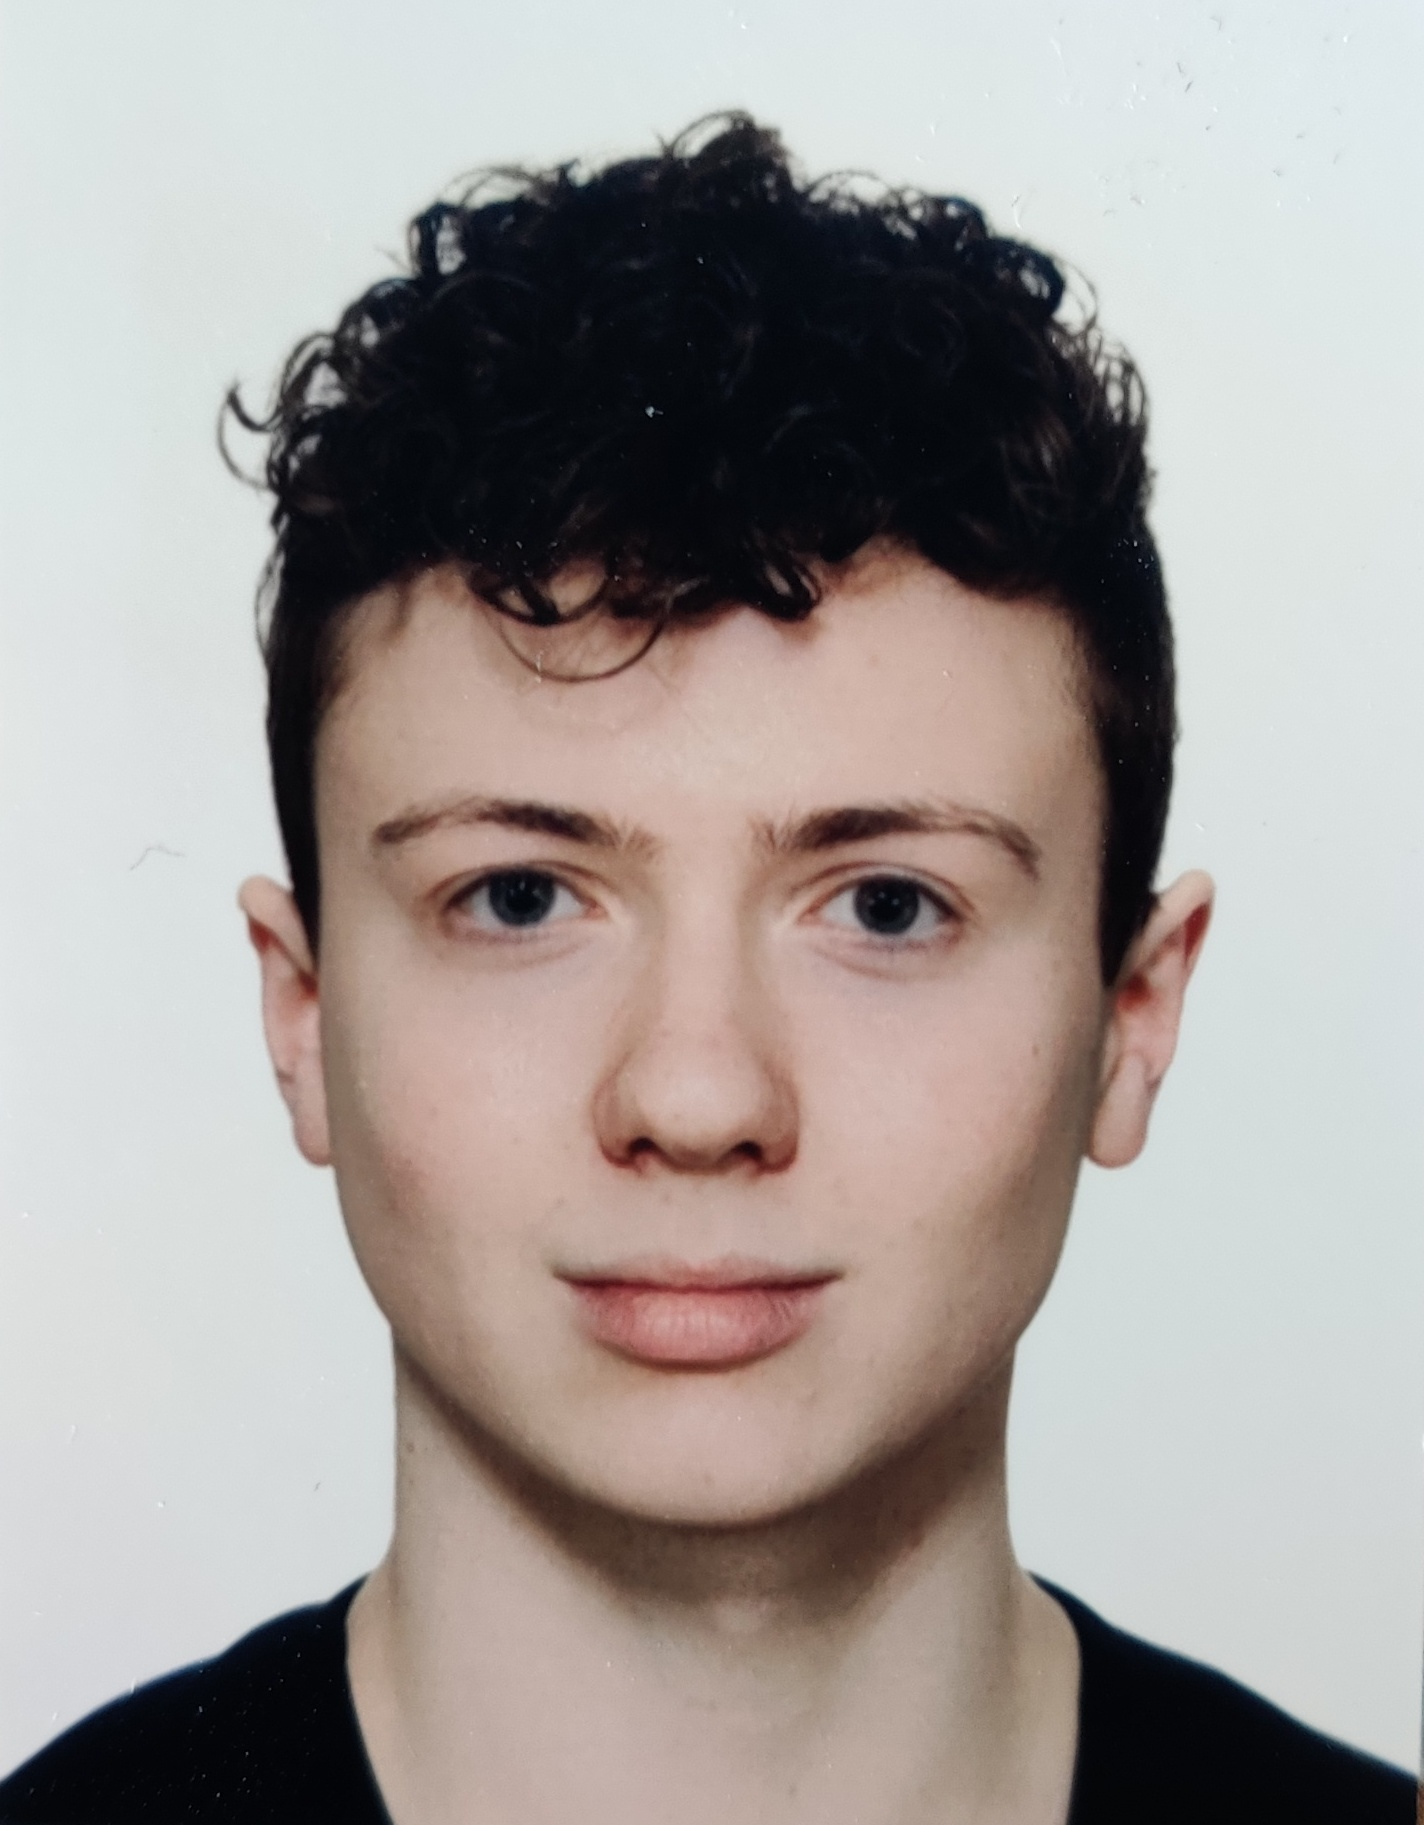
\includegraphics[width=3cm, right]{./Portrait.jpg}} \\\\[-4pt]%[8pt]
    \href{tel:+4551164199}{\faIcon{mobile-alt}~\large~+45 51 16 41 99} \\\\[-4pt]%[8pt] 
    \href{https://github.com/LohseBoi}{\faIcon{github}~\footnotesize\faIcon{at}\large \texttt{LohseBoi}} \\\\[-4pt]%[8pt]
    \href{https://gitlab.com/LohseBoi}{\faIcon{gitlab}~\footnotesize\faIcon{at}\large \texttt{LohseBoi}} \\\\[-4pt]%[8pt]
    %\href{mailto:thomas.k.lohse@gmail.com}{\faIcon{envelope}~\large thomas.k.lohse\normalsize\MVAt\large gmail.com} \\\\[7pt]%[-4pt]%[8pt]
    \href{mailto:thomas.k.lohse@gmail.com}{\faIcon{envelope}~\large thomas.k.lohse\normalsize\MVAt\large gmail.com} \\\\[-4pt]%[8pt]
    \href{https://linkedin.com/in/thomas-lohse}{\faIcon{linkedin}~\large LinkedIn}\\\\[-14pt]
    \bottomrule
\end{tabular}
%\par\noindent\rule{\textwidth}{1pt}

    \section*{Uddannelse}
    %\lipsum[4]\\[0.5cm]
    \begin{tabular}{r|p{.82\linewidth}} 
        2007--2016 & \textbf{Folkeskole}\\
    &   Elev på Vodskov Skole til og med ottende klasse.
        \\\\
        2016--2017 & \textbf{Efterskole}\\
    &   Elev på Ingstrup Efterskole i niende klasse.
        \\\\
        2017--2020 & \textbf{Gymnasie}\\
    &   Elev på Aalborg Techcollege (AATG), hvor jeg tog den tekniske studentereksamen (HTX),
        med profilfagende \textit{Kommunikation \& IT} A og \textit{Programmering} B, samt teknikfag i \textit{Elektronisk Udvikling og Produktion} A.
        \\\\
        2020--Nu & \textbf{Universitet}\\
    &   Software Ingeniør, Bachelor studerende på Aalborg Universitet.
    \end{tabular}
 
    \section*{Beskæftigelse \& Anden Erfaring}
    \subsection*{Beskæftigelse}
    \begin{tabular}{r|p{.82\linewidth}}%TODO
        2018--2019 & \textbf{Føtex Nørresundby}\\
    &   I løbet af min ansættelse hos Føtex Nørresundby, havde jeg en mindre mængde af stillinger:
        \begin{itemize}\setlength\itemsep{0em}
            \item[] \textbf{Servicemedarbejder --- } Min første kontrakt var under stillingen 
                Servicemedarbejder, som havde et udvalg af opgaver, hvor den primære var at
                opretholde pantflaskemaskinerne.
            \item[] \textbf{Kasse Assistent --- } Omkring et halvt år efter min ansættelse, bliver
                jeg tilbudt en oplæring og ny tilhørende stilling som Kasse Assistent.
            \item[] \textbf{Bake-Off Sal --- } Da jeg fylder 18 år, og min kontrakt opsiges,
                tilbyder de mig en ny kontrakt med stillingen Bake-Off Salsperson, som var min stilling
                op til min opsigelse.
        \end{itemize}
    \end{tabular}

    \subsection*{Anden Erfaring}
    \begin{tabular}{r|p{.82\linewidth}}
        2021--Nu & \textbf{UNF Game Development Camp}\\
    &   Jeg er frivillig medarbedjer hos UNFs Game Development Camp, hvor jeg har haft de følgdende roller:
        \begin{itemize}\setlength\itemsep{0em}
            \item[2021] \textbf{Programmingsassistent ---} Assistere programmeringslæren, samt hjælp
                med deltagernes programmeringsrelateret problemer.
            \item[2021] \textbf{Logistisk Ansvarlig ---} Ansvarlig for håndtering af det logistiken
                vedrørende de frivilliges anmodninger om vare, samt anskaffelsen.
            \item[2021] \textbf{Teknisk Ansvarlig ---} Ansvarlig for alt udstyret til campen, samt
                introduktionen af \verb|git| for deltagerne, og håndtering af alle problemer de
                måtte have med al det tekniske.
        \end{itemize}
        \\
        2021 & \textbf{Tutor}\\
    &   Jeg var frivillig tutor for de nye Software, Bachelor studerende på Aalborg Universitet.
    \end{tabular}

    \section*{Fritidsaktiviter/Hobbies}
    \begin{itemize}\setlength\itemsep{0.5em}
        \item[] \textbf{IT}\\
            Jeg laver mine egne små programmingsprojekter/-opgaver, samt configurering og fumleri
            med mit Linux-system, og firmware design til mit tastatur.
        \item[] \textbf{Programmingsungdomsklub}\\
            Om tirsdagem er jeg i en programmingsungdomsklub kaldet GameLab, som er styret af
            UngAalborg.
        \item[] \textbf{Fysisk Aktivitet}\\
            Jeg sørger for at være fysisk aktiv, primært i formen af styektræning i et fitness center.
    \end{itemize}

    \section*{Referencer}
    Fremsendes efter anmodning.
\iffalse
    \begin{tabular}{r|p{.82\linewidth}}
        Føtex Nørresundby & \textbf{Sabine Them}                                \\
        &\href{tel:+4522469893}
            {\faIcon{mobile-alt}~+45 22 46 98 93}                               \\
        &\href{mailto:sabine.them@foetex.dk}
            {\faIcon{envelope}~sabine.them\small\MVAt\normalsize foetex.dk}     \\[.3cm]
        Føtex Nørresundby & \textbf{Joan Jørgensen}                             \\
        &\href{tel:+4522760661}
            {\faIcon{mobile-alt}~+45 22 72 06 61}                               \\
        &\href{mailto:joan.joergensen@foetex.dk}
            {\faIcon{envelope}~joan.joergensen\small\MVAt\normalsize foetex.dk} \\[.3cm]
        GameLab UngAalborg & \textbf{Christian "Code" Skriver Kragegaard}       \\
        &\href{tel:+4593520910}
            {\faIcon{mobile-alt}~+45 93 52 09 10}                               \\
        &\href{mailto:Csk-skole@ungaucnet.dk}
            {\faIcon{envelope}~Csk-skole\small\MVAt\normalsize ungaucnet.dk}    \\
    \end{tabular}
\fi

\end{document}

